% Created by tikzDevice version 0.10.1 on 2016-04-06 15:10:52
% !TEX encoding = UTF-8 Unicode
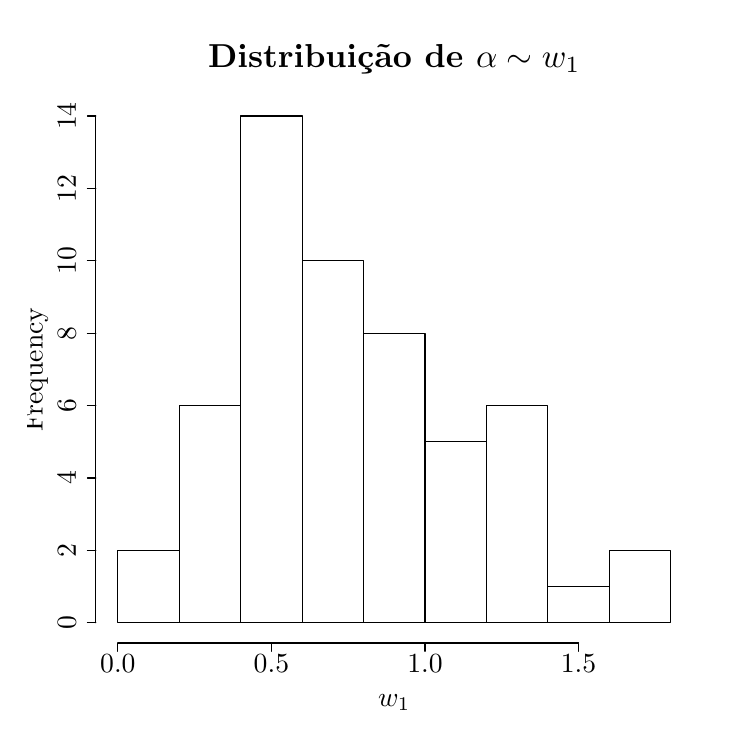
\begin{tikzpicture}[x=.5pt,y=.5pt]
\definecolor{fillColor}{RGB}{255,255,255}
\path[use as bounding box,fill=fillColor,fill opacity=0.00] (0,0) rectangle (505.89,505.89);
\begin{scope}
\path[clip] (  0.00,  0.00) rectangle (505.89,505.89);
\definecolor{drawColor}{RGB}{0,0,0}

\node[text=drawColor,anchor=base,inner sep=0pt, outer sep=0pt, scale=  1.20] at (264.94,477.15) {\bfseries Distribuição de $\alpha \sim w_1$};

\node[text=drawColor,anchor=base,inner sep=0pt, outer sep=0pt, scale=  1.00] at (264.94, 15.60) {$w_1$};

\node[text=drawColor,rotate= 90.00,anchor=base,inner sep=0pt, outer sep=0pt, scale=  1.00] at ( 10.80,258.94) {Frequency};
\end{scope}
\begin{scope}
\path[clip] (  0.00,  0.00) rectangle (505.89,505.89);
\definecolor{drawColor}{RGB}{0,0,0}

\path[draw=drawColor,line width= 0.4pt,line join=round,line cap=round] ( 65.18, 61.20) -- (398.12, 61.20);

\path[draw=drawColor,line width= 0.4pt,line join=round,line cap=round] ( 65.18, 61.20) -- ( 65.18, 55.20);

\path[draw=drawColor,line width= 0.4pt,line join=round,line cap=round] (176.16, 61.20) -- (176.16, 55.20);

\path[draw=drawColor,line width= 0.4pt,line join=round,line cap=round] (287.14, 61.20) -- (287.14, 55.20);

\path[draw=drawColor,line width= 0.4pt,line join=round,line cap=round] (398.12, 61.20) -- (398.12, 55.20);

\node[text=drawColor,anchor=base,inner sep=0pt, outer sep=0pt, scale=  1.00] at ( 65.18, 39.60) {0.0};

\node[text=drawColor,anchor=base,inner sep=0pt, outer sep=0pt, scale=  1.00] at (176.16, 39.60) {0.5};

\node[text=drawColor,anchor=base,inner sep=0pt, outer sep=0pt, scale=  1.00] at (287.14, 39.60) {1.0};

\node[text=drawColor,anchor=base,inner sep=0pt, outer sep=0pt, scale=  1.00] at (398.12, 39.60) {1.5};

\path[draw=drawColor,line width= 0.4pt,line join=round,line cap=round] ( 49.20, 75.85) -- ( 49.20,442.04);

\path[draw=drawColor,line width= 0.4pt,line join=round,line cap=round] ( 49.20, 75.85) -- ( 43.20, 75.85);

\path[draw=drawColor,line width= 0.4pt,line join=round,line cap=round] ( 49.20,128.16) -- ( 43.20,128.16);

\path[draw=drawColor,line width= 0.4pt,line join=round,line cap=round] ( 49.20,180.47) -- ( 43.20,180.47);

\path[draw=drawColor,line width= 0.4pt,line join=round,line cap=round] ( 49.20,232.79) -- ( 43.20,232.79);

\path[draw=drawColor,line width= 0.4pt,line join=round,line cap=round] ( 49.20,285.10) -- ( 43.20,285.10);

\path[draw=drawColor,line width= 0.4pt,line join=round,line cap=round] ( 49.20,337.42) -- ( 43.20,337.42);

\path[draw=drawColor,line width= 0.4pt,line join=round,line cap=round] ( 49.20,389.73) -- ( 43.20,389.73);

\path[draw=drawColor,line width= 0.4pt,line join=round,line cap=round] ( 49.20,442.04) -- ( 43.20,442.04);

\node[text=drawColor,rotate= 90.00,anchor=base,inner sep=0pt, outer sep=0pt, scale=  1.00] at ( 34.80, 75.85) {0};

\node[text=drawColor,rotate= 90.00,anchor=base,inner sep=0pt, outer sep=0pt, scale=  1.00] at ( 34.80,128.16) {2};

\node[text=drawColor,rotate= 90.00,anchor=base,inner sep=0pt, outer sep=0pt, scale=  1.00] at ( 34.80,180.47) {4};

\node[text=drawColor,rotate= 90.00,anchor=base,inner sep=0pt, outer sep=0pt, scale=  1.00] at ( 34.80,232.79) {6};

\node[text=drawColor,rotate= 90.00,anchor=base,inner sep=0pt, outer sep=0pt, scale=  1.00] at ( 34.80,285.10) {8};

\node[text=drawColor,rotate= 90.00,anchor=base,inner sep=0pt, outer sep=0pt, scale=  1.00] at ( 34.80,337.42) {10};

\node[text=drawColor,rotate= 90.00,anchor=base,inner sep=0pt, outer sep=0pt, scale=  1.00] at ( 34.80,389.73) {12};

\node[text=drawColor,rotate= 90.00,anchor=base,inner sep=0pt, outer sep=0pt, scale=  1.00] at ( 34.80,442.04) {14};
\end{scope}
\begin{scope}
\path[clip] ( 49.20, 61.20) rectangle (480.69,456.69);
\definecolor{drawColor}{RGB}{0,0,0}

\path[draw=drawColor,line width= 0.4pt,line join=round,line cap=round] ( 65.18, 75.85) rectangle (109.57,128.16);

\path[draw=drawColor,line width= 0.4pt,line join=round,line cap=round] (109.57, 75.85) rectangle (153.97,232.79);

\path[draw=drawColor,line width= 0.4pt,line join=round,line cap=round] (153.97, 75.85) rectangle (198.36,442.04);

\path[draw=drawColor,line width= 0.4pt,line join=round,line cap=round] (198.36, 75.85) rectangle (242.75,337.42);

\path[draw=drawColor,line width= 0.4pt,line join=round,line cap=round] (242.75, 75.85) rectangle (287.14,285.10);

\path[draw=drawColor,line width= 0.4pt,line join=round,line cap=round] (287.14, 75.85) rectangle (331.53,206.63);

\path[draw=drawColor,line width= 0.4pt,line join=round,line cap=round] (331.53, 75.85) rectangle (375.92,232.79);

\path[draw=drawColor,line width= 0.4pt,line join=round,line cap=round] (375.92, 75.85) rectangle (420.32,102.00);

\path[draw=drawColor,line width= 0.4pt,line join=round,line cap=round] (420.32, 75.85) rectangle (464.71,128.16);
\end{scope}
\end{tikzpicture}
